\documentclass[xetex,mathserif,serif]{beamer}
\usepackage{polyglossia}
\setdefaultlanguage[babelshorthands=true]{russian}
\usepackage{minted}
\usepackage{tabu}

\useoutertheme{infolines}

\usepackage{fontspec}
\setmainfont{FreeSans}
\newfontfamily{\russianfonttt}{FreeSans}

\definecolor{links}{HTML}{2A1B81}
\hypersetup{colorlinks,linkcolor=,urlcolor=links}

\tabulinesep=0.7mm

\newcommand{\attribution}[1] {
    \vspace{-5mm}\begin{flushright}\begin{scriptsize}\textcolor{gray}{\textcopyright\, #1}\end{scriptsize}\end{flushright}
}

\title{Практика 2: Практика по визуальному моделированию}
\subtitle{Часть 1: Анализ}
\author[Юрий Литвинов]{Юрий Литвинов\\\small{\textcolor{gray}{y.litvinov@spbu.ru}}}

\date{17.03.2022}

\begin{document}

    \frame{\titlepage}

    \begin{frame}
        \frametitle{Напоминание, диаграмма случаев использования UML}
        \begin{columns}
            \begin{column}{0.6\textwidth}
                \begin{itemize}
                    \item Акторы (или актёры, роли) --- внешние сущности, использующие систему
                    \begin{itemize}
                        \item Люди или другие программные системы
                    \end{itemize}
                    \item Случаи использования (прецеденты)  --- цель использования системы актором
                    \begin{itemize}
                        \item Одно-два слова о цели использования
                        \item \textit{Не последовательность действий}
                        \item \textit{Не модель данных}
                    \end{itemize}
                    \item Цель: определиться с количеством и функциональностью АРМ
                \end{itemize}
            \end{column}
            \begin{column}{0.4\textwidth}
                \begin{center}
                    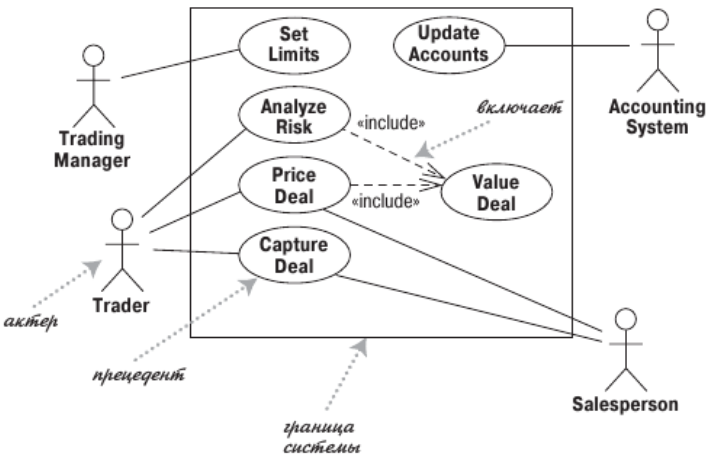
\includegraphics[width=\textwidth]{useCaseDiagram.png}
                    \attribution{М. Фаулер, UML. Основы}
                \end{center}
            \end{column}
        \end{columns}
    \end{frame}

    \begin{frame}
        \frametitle{Напоминание, диаграмма активностей}
        \begin{columns}
            \begin{column}{0.5\textwidth}
                \begin{itemize}
                    \item Модель бизнес-процесса
                    \item Как раз тут --- последовательность действий, но без привязки к конкретной системе
                    \item \url{https://www.uml-diagrams.org/activity-diagrams.html}
                    \item Обратите внимание на синтаксис ветвлений
                    \item Пользуйтесь дорожками
                \end{itemize}
            \end{column}
            \begin{column}{0.5\textwidth}
                \begin{center}
                    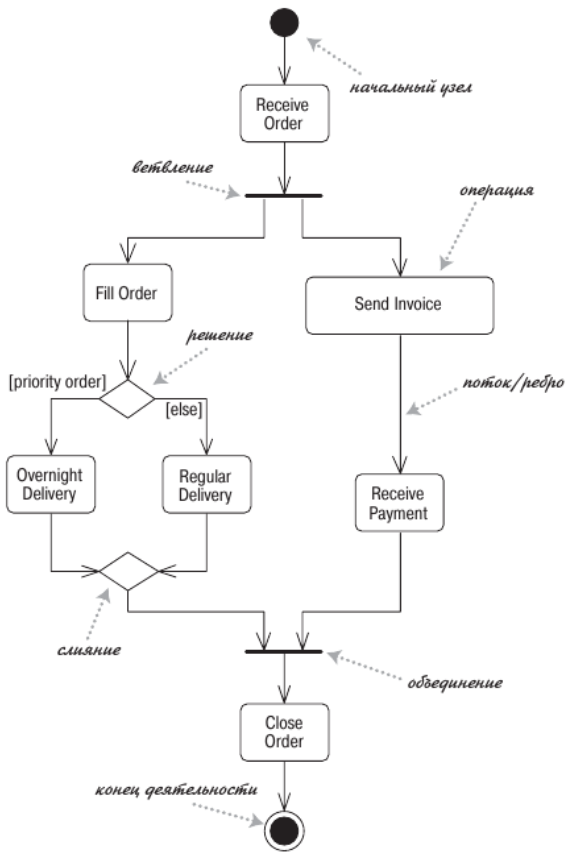
\includegraphics[width=0.7\textwidth]{activityDiagram.png}
                    \attribution{М. Фаулер, UML. Основы}
                \end{center}
            \end{column}
        \end{columns}
    \end{frame}

    \begin{frame}
        \frametitle{Задачи на пару}
        \begin{itemize}
            \item Проанализировать запрос \url{https://goo.gl/MiyH8c}
            \item Задача 1: Нарисовать диаграмму случаев использования разрабатываемого приложения
            \item Задача 2: Нарисовать диаграмму активностей для бизнес-процесса предприятия, для которого разрабатывается приложение
            \item Пользоваться одним из CASE-инструментов с лекции
            \begin{itemize}
                \item \url{https://app.diagrams.net/}
                \item Расшарьте проект сразу, я буду комментировать по ходу
            \end{itemize}
            \item Отчуждаемый результат --- ссылка на проект с диаграммой в решение в MS Teams
            \begin{itemize}
                \item Не забудьте расшарить
            \end{itemize}
            \item В 16:50 встречаемся в общем чате и показываем пару решений
        \end{itemize}
    \end{frame}

\end{document}
